\chapterillustration{./abertura-documentacao}{./abertura-documentacao-professor}

\chapterwhat{O Livro Aberto de Matemática é um projeto de construção de um material didático de matemática de distribuição livre e \textit{Open Source}, isto é, o código é aberto e pode receber submissões de qualquer um que deseje colaborar}

\chapterbecause{O Esforço para produzir livros didáticos de Matemática com licença aberta começou em 2016, com a elaboração do material de Frações para o ensino fundamental I. Desde então, novos elaboradores acreditaram e juntaram-se ao projeto para alcançarmos novos níveis e novos livros. Hoje, possuímos diversos capítulos escritos e outros 6 livros em produção. Tudo isso a partir de um trabalho colaborativo envolvendo matemáticos, professores universitários e professores da Educação Básica.

Um princípio fundamental desta iniciativa é que sua produção configure uma proposta pedagógica ancorada e acompanhada por pesquisa científica em Ensino de Matemática. O projeto tem também compromisso com a formação e o desenvolvimento profissional de professores. Em particular, pela composição característica da equipe, destaca-se o entendimento do potencial do projeto para enfrentar um reconhecido desafio: estreitar o diálogo entre a realidade e as demandas próprias da prática docente e a formação acadêmica do professor. Leia mais a respeito. Você também pode sugerir alterações no texto do projeto pelo \href{https://github.com/livro-aberto/tex-design-development}{Github}.}


\chapter{Documentação do Livro Aberto do Ensino Médio}

\autorum{Tarso Boudet Caldas}

\ilustracao{Miller  Guglielmo}

\versao{0.5}

\autordacapa{Bernd Klutsch}{Unplash}{https://unsplash.com/photos/nE2HV5AUXFo}

\creditos

\mainmatter


% \begin{apresentacao}{Introdução à Documentação do Material do Professor}
% A versão do professor atual possui algumas diferenças em relação ao material do aluno, mas utilizando o mesmo arquivo do capítulo em \verb|.tex|. Isto quer dizer que para gerar o material, o texto do capítulo do aluno e do professor convivem no mesmo arquivo, apenas com a diferença de que se compila o arquivo \verb|professor.tex| em vez do \verb|aluno.tex|. De resto, as recomendação sobre como compilar esse texto \textbf{as mesmas} do \textcolor{session1}{Explorando: O que é necessário?} no início desta documentação. Com as seguintes diferenças:
% \begin{itemize}
% \item Ao adicionar a figura de abertura do capítulo, deve haver duas versões, uma para a do aluno e outra para a do professor. Como o tamanho da página do arquivo do aluno é diferente da do professor, as imagens de abertura possuem tamanhos diferentes. A abertura do aluno está no formato proporcional a \verb|2000 x 2924| pixels e do professor a \verb|2000 x 1646| pixels. É importante observar que as imagens não precisam estar nestes números, apenas deve ter o tamanho proporcional, caso contrário a imagem da capa ficará distorcida.

% \item Há novos ambientes e comandos para os textos do professor, que serão melhor explicados adiantes.
% \end{itemize}

% Para gerar uma página como esta de apresentação, usamos o ambiente
% \begin{verbatim}
% \begin{apresentacao}{titulo}

% \end{apresentacao}
% \end{verbatim}
% com o título de apresentação de sua escolha.  

% É possível também criar uma página de texto para o professor como a da apresentação no meio do texto, que pode ser utilizada como transição entre seções. O ambiente é \verb|paginatexto|. Há mais à frente neste texto um \hyperref[paginatexto]{exemplo do ambiente}

% \subsection{Limitações}
% Por ser uma versão beta do modelo, alguns problemas podem surgir no uso. Este é feito com base em margens, isto é, o material do aluno é o texto principal e o material do professor as margens deste material. Por este motivo, há a dificuldade de alinhamento das caixas do professor nas páginas, por isso, algumas "gambiarras"{} devem ser feitas para que o alinhamento ocorra de modo desejado. Estas serão explicadas no máximo de suas possibilidades, mas alguns problemas podem surgir. 

% Ao encontrar um erro, pedimos que este seja reportado na seção de \href{https://github.com/livro-aberto/tex-design-development/issues}{"issues"{} no GitHub do projeto}, para que estes possam ser visto pelo maior número de pessoas, ajudando aqueles que encontrarem um erro semelhante, e também para que os colaboradores que souberem como solucionar o problema tenham melhor acesso.

% A seguir iremos descrever os ambientes novos criados e seguiremos a exemplificar nas próximas páginas.

% \subsection{Habilidades}
% Temos o ambiente \verb|habilities|, como no exemplo a seguir:

% \begin{habilities}{EM13MAT305}
% Resolver e elaborar problemas com funções logarítmicas nos quais seja necessário compreender e interpretar a variação das grandezas envolvidas, em contextos como os de abalos sísmicos, pH, radioatividade, Matemática Financeira, entre outros.
% \tcbsubtitle{EM13MAT403}
% Analisar e estabelecer relações, com ou sem apoio de tecnologias digitais, entre as representações de funções exponencial e logarítmica expressas em tabelas e em plano cartesiano, para identificar as características fundamentais (domínio, imagem, crescimento) de cada função.
% \end{habilities}

% Estas são as habilidades, do capítulo de Logaritmos. Este ambiente foi gerado pelo seguinte código:
% \begin{verbatim}
% \begin{habilities}{EM13MAT305}
% texto da habilidade

% \tcbsubtitle{EM13MAT403}
% texto da habilidade
% \end{habilities}
% \end{verbatim}

% A primeira habilidade deve estar entre chaves logo depois do início do ambiente. Se houver outras habilidades a serem colocadas no mesmo ambiente, o título deve estar no comando \verb|\tcbsubtitle{habilidade}|. Não há limite para o número de habilidades.

% \subsection{Caixas do para o professor}

% O conteúdo para a descrição dos objetivos, sugestões e soluções de atividades e afins deve ser colocado nas seguintes caixas

% \paragraph{Objetivos Específicos}
% Para descrever os objetivos específicos de uma atividade, utilizamos o ambiente \verb|objectives|, com os seguintes argumentos:
% \begin{verbatim}
% \begin{objectives}{título}
% {
% conteúdo
% }{lado da página}{notas}
% \end{objectives}
% \end{verbatim}
% Além do título e do conteúdo, o ambiente requer dois números, um para o lado da página, isto é, se é uma página par ou ímpar. No caso de página ímpar, usamos o número \verb|1| e para páginas ímpar o número \verb|2|. O segundo número indica se a caixa será colocada na página (\verb|1|) do conteúdo ou na seção das notas no final do capítulo (\verb|0|) (exemplificaremos mais à frente). Recomenda-se não colocar os objetivos específicos nas notas no final do capítulo, a menos que necessário.

% \paragraph{Sugestões e discussões}
% Nesta caixa escrevemos informações úteis à execução de uma atividade ou para chamar a atenção a algum conteúdo da página. O funcionamento é o mesmo da caixa de objetivos específicos, mas com o nome \verb|sugestions|:
% \begin{verbatim}
% \begin{sugestions}{título}
% {
% conteúdo
% }{lado da página}{notas}
% \end{sugestions}
% \end{verbatim}
% Neste caso, as notas têm três possibilidades: \verb|1|, \verb|0| ou \verb|9|. A diferença entre a caixa de objetivos específicos e de sugestões é a opção de quebra de página da caixa ao final do capítulo. Traremos exemplos mais tarde.

% \paragraph{Respostas}
% \begin{verbatim}
% \begin{answer}{título}
% {
% conteúdo
% }{notas}
% \end{answer}
% \end{verbatim}
% O ambiente de respostas não possui diferenciação no lado da página, mas possui o mesmo argumento sobre as notas no final do capítulo que o ambiente de sugestões.

% \paragraph{Texto fora da caixa}
% Para escrever texto nas margens da página, que não as caixas citadas acima, pode-se utilizar o ambiente \verb|texto|:
% \begin{verbatim}
% \begin{texto}
% {
% conteúdo
% }
% \end{texto}
% \end{verbatim}

% \subsection{Posicionamento das caixas no código}

% Por conflitos com as outras caixas do material do aluno, o conteúdo das margens tem sido colocado \textbf{antes} das seções Explorando e afins. A quebra de página das margens deve ser feita com o comando \verb|\clearmargin|, que tem a mesma funcionalidade de \verb|\clearpage|, mas apenas para a margem.

% Por exemplo:
% \begin{verbatim}
% \def\currentcolor{session1}
% \begin{objectives}{atividade 1}
% {

% }{1}{1}
% \end{objectives}
% \begin{sugestions}{atividade 1}
% {

% }{1}{1}
% \end{sugestions}
% \clearmargin
% \begin{answer}{atividade 1}
% {

% }{1}
% \end{answer}
% \explore{título}
% \end{verbatim}

% Neste caso, teríamos a definição da cor da caixa usando \verb|\def\currentcolor{cor}|. Suas opções são 
% \begin{itemize}
% \item \verb|session1|, a cor do \textcolor{session1}{Explorando} 
% \item \verb|session2|, a cor do \textcolor{session2}{Praticando}
% \item \verb|session3|, a cor do \textcolor{session3}{Para Saber+}
% \item \verb|session4|, a cor do \textcolor{session4}{Organizando} e
% \item \verb|cor1|, a cor dos \textcolor{cor1}{Exercícios}
% \item \verb|cor1|, a cor do \textcolor{cor2}{Projeto aplicado}
% \end{itemize}


% \subsection{Considerações}


% \paragraph{Adjustbox}
% As opções das notas no final do capítulo dizem respeito à quebra ou não da \verb|tcolorbox|. Quando permitido que as caixas quebrem, há a possibilidade da caixa ir para a próxima página enquando o marcador da nota fique na anterior. Por este motivo é usado o pacote e o comando \verb|adjustbox|. Com ele é possível alinhar a caixa ao marcador da nota. Entretanto, quando é usado este comando a caixa perde a possibilidade de quebrar, por isso é necessário atenção ao utilizar os comandos. 

% Nos casos das três caixas de objetivos, sugestões e respostas, o último número a ser colocado é \verb|1| se é desejado que a caixa apareça na própria página; \verb|0| se é desejado que vá para as notas (usando \verb|adjustbox|) e \verb|9| quando se deseja que a caixa quebre (sem \verb|adjustbox|). Vamos mostrar casos das duas possibilidades.

% \paragraph{Marcadores de texto no PDF}

% Apesar de não termos ainda um sumário estruturado, as seções geram marcadores de texto (\textit{Bookmarks}) no PDF. Capítulos diferentes possuem estruturas diferentes, e por isso temos um comando para alterar a hierarquia das seções nos marcadores: \verb|\expandtocdepth|.

% A estrutura padrão é:

% \begin{Verbatim}
% \chapter
%   \section (a apresentação e a pagina de texto no meio do capítulo são definidas a partir deste comando)
%   \explore
%   \arrange
%   \practice
%   \know
%   \exercise
%   Notas
% \end{Verbatim}

% Ou seja, todas as seções ficam com a mesma hierarquia. Com \verb|\expandtocdepth| o Explorando, o Organizando e o Praticando ficam abaixo das seções:

% \begin{Verbatim}
% \chapter
%   \section
%     \explore
%     \arrange
%     \practice
%   \know
%   \exercise
%   Notas
% \end{Verbatim}

% É possível colocar também os comandos \verb|\know| e \verb|\exercise| abaixo das seções, colocando as opções \verb|know| e/ou \verb|exercise| como opção. Isto é, \verb|\expandtocdepth[know]| gerará a estrutura

% \begin{Verbatim}
% \chapter
%   \section
%     \explore
%     \arrange
%     \practice
%     \know
%   \exercise
%   Notas
% \end{Verbatim}

% \end{apresentacao}

\def\currentcolor{session1}
\begin{objectives}{Título da atividade}
{Esta caixa foi criada usando o comando 
\texttt{\textbackslash begin\{objectives\}\{Título da atividade\}\newline
\{\newline
Conteúdo\newline
\}\{1\}\{1\}\newline
\textbackslash end\{objectives\}
}


Como no terceiro argumento da caixa usamos ``\texttt{1}'', ela ficará na página no meio do texto. Se usarmos ``\texttt{0}'', ela irá então para o final do capítulo, criando uma ``Nota'', como você pode observar abaixo desta caixa.
}{1}{1}
\end{objectives}


\begin{objectives}{Título da atividade}
{
Esta caixa foi criada usando ``\texttt{0}'' no terceiro argumento.

\texttt{\textbackslash begin\{objectives\}\{Título da atividade\}\newline
\{\newline
Conteúdo\newline
\}\{0\}\{1\}\newline
\textbackslash end\{objectives\}
}

Vale notar que se a caixa está no final das notas, o quarto argumento perde função.
}{0}{1}
\end{objectives}
\clearmargin
\begin{sugestions}{Título da atividade}
{
Usando o comando \texttt{\textbackslash clearmargin}, pulamos para a próxima página do texto, e utilizamos na caixa de sugestões o quarto argumento ``\texttt{0}'' para acomodá-la na página par (meramente visual). Isto faz o visual para o texto no modo de leitura de livro (recomedamos este modo de visualização).
\texttt{\textbackslash begin\{sugestions\}\{Título da atividade\}\newline
\{\newline
Conteúdo\newline
\}\{1\}\{0\}\newline
\textbackslash end\{sugestions\}
}
}{1}{0}
\end{sugestions}
\begin{answer}{Título da atividade}
{
\begin{enumerate}
\item O mesmo valerá para a caixa de resposta, ao utilizar ``1'' no terceiro argumento teremos ela ao lado do texto, mas se utilizarmos ``0''
\end{enumerate}
}{1}
\end{answer}

\begin{answer}{Caixas nas notas com muito texto}
{
\textbf{Se temos um texto muito grande em caixas que vão para as notas no final do capítulo, ao usarmos ``\texttt{0}'' no terceiro argumento, a caixa não conseguirá quebrar para a próxima coluna, como no caso que temos aqui.}

\lipsum
}{0}
\end{answer}

\begin{answer}{Caixas nas notas com muito texto}
{
\textbf{Por este motivo, é possível utilizar ``\texttt{9}'' no terceiro argumento (isto também vale para a caixa de objetivos e de sugestões), o que permitirá que a caixa quebre. É importante ressaltar que isso pode fazer com que o número ao lado da caixa que indica o número da nota pode ficar numa página diferente quando usamos esta versão, entre outros efeitos indesejados de quebra de coluna, como no caso que temos aqui, por isso é necessário ter cautela ao utilizar esta variante.}

\lipsum
}{9}
\end{answer}


\explore{O que é necessário?}

Para a utilização deste pacote é necessário os arquivos que estão incluídos no repositório \verb|tex-design-development| no \href{https://github.com/livro-aberto/tex-design-development/}{GitHub} do projeto. Os arquivos são:
\begin{itemize}
\item O diretório \verb|chapters/|, onde devem ser colocados os capítulos em produção (nele estão exemplos de outros capítulos já produzidos, mas estes arquivos não são necessários).
\item O diretório \verb|Figuras/|, onde devem ser colocadas as figuras dos capítulos (estão incluídas no GitHub uma pasta com as figuras de todos os capítulos produzidos até o momento e também uma pasta apenas com as figuras necessárias para a geração de um capítulo novo).
\item O diretório \verb|Fontes/| que possui todas as fontes usadas no livro (elas devem ser instaladas na sua máquina).
\item Os pacotes \verb|sphinx.sty|, \verb|livroaberto.sty| e \verb|livroaberto-professor.sty|.
\item O arquivo \verb|aluno.tex| para a compilação do material do aluno e o arquivo \verb|professor.tex| para compilar o material do professor.
\end{itemize}

Todos estes arquivos estão presentes nas pastas \verb|Minimal.zip| ou \verb|Minimal.tar|.

Além disso, é necessário ter instalado a versão mais recente do \href{https://www.tug.org/texlive/}{\TeX{} Live} \textbf{ou} \href{https://miktex.org/}{Mik\TeX}{} (preferencialmente suas devidas versões completas) e um editor de texto à sua escolha. Não pretendemos a ensinar o uso de \LaTeX, mas mostrar a estrutura e padronização utilizada nos capítulos já existentes do projeto. Para aqueles que possuem interesse em aprender indicamos \href{http://www.uft.edu.br/engambiental/prof/catalunha/arquivos/latex/latex_GilbertoSouto.pdf}{Curso de \LaTeX{}} de Gilberto Souto. %provisório


\subsection{Início do capítulo}

Para começar o seu capítulo e poder compilá-lo, é necessário editar no arquivo \verb|aluno.tex| ou \verb|professor.tex|, dependendo de qual versão se deseje compilar, após o início do documento, incluindo o nome do seu arquivo pelo comando \verb|\include{chapters/seucapitulo}| (lembrando que o arquivo deve estar na pasta \verb|/chapters|). É necessário usar \verb|xelatex| para compilar propriamente.

No início do arquivo de seu capítulo é preciso colocar o que seria o "preâmbulo"{} do capítulo, isto é, antes do primeiro explorando é preciso colocar a abertura e os créditos (isto pode ser feito copiando de outro capítulo já pronto). A partir disso, é necessário:

\begin{itemize}
\item A ilustração da capa, que pode ser feito alterando o comando \spverb|\chapterillustration{./abertura-capitulo}{.abertura-capitulo-professor||. A capa deve estar na pasta \verb|/Figuras| e deve ter o nome no formato \spverb|abertura-nomedocapitulo|. A figura deve ter licença gratuita, e deve ser preferencialmente no formado de retrato. Figuras gratuitas podem ser encontradas no site \href{https://unsplash.com/}{Unsplash}.

\item O "O Quê?"{} pode ser colocado dentro comando \spverb|\chapterwhat{o que}|; o "Por Quê"{} em \spverb|\chapterbecause{por que}| e o nome do capítulo em \spverb|\chapter{capitulo}|

\item Alterar na página de créditos a partir dos seguintes comandos:
\begin{enumerate}
\item \verb|\autorum|, \verb|autordois|, ..., \verb|autorcinco| para o nome dos autores (até cinco nomes).
\item \verb|\revisorum|, \verb|revisordois|, ..., \verb|revisorcinco| para o nome dos revisores (até cinco nomes).
\item \verb|\versao| a versão atual do material.
\item \verb|\graficos| para o nome do(a) autor(a) de figuras técnicas.
\item \verb|\ilustracao| para o nome do(a) ilustrador(a).
\item \verb|\autordacapa{Autor}{Fonte}{Link}| para os créditos da imagem de capa. Este comando coloca a frase ``Foto de Autor no Fonte'' na página de créditos, onde fonte é o site de retirada da imagem.
\end{enumerate}

Entre todos estes comandos, apenas o nome do primeiro autor e a versão são necessários para que não haja erro. Para então criar a página de créditos é necessário usar o comando \verb|\creditos| após as definições acima.
\end{itemize}

Após isso, basta começar o Explorando após \verb|\mainmatter| usando \verb|\explore{nome da seção}|.

\begin{task}{Caixa de atividade}

A primeira parte de uma seção é o Explorando. Nela são colocadas atividades que introduzem o assunto que será discutido. Para criar uma caixa de atividade usamos
\begin{verbatim}
\begin{task}{Título da atividade}

Texto da atividade

\end{task}
\end{verbatim} 

O comando \verb|\label| também pode ser usado na caixa de atividade.
\end{task}


\begin{task}{Figuras}
Na sua atividade, você pode querer incluir figuras e tabelas. Temos um padrão que para essa inclusão.

\begin{figure}[H]
\centering

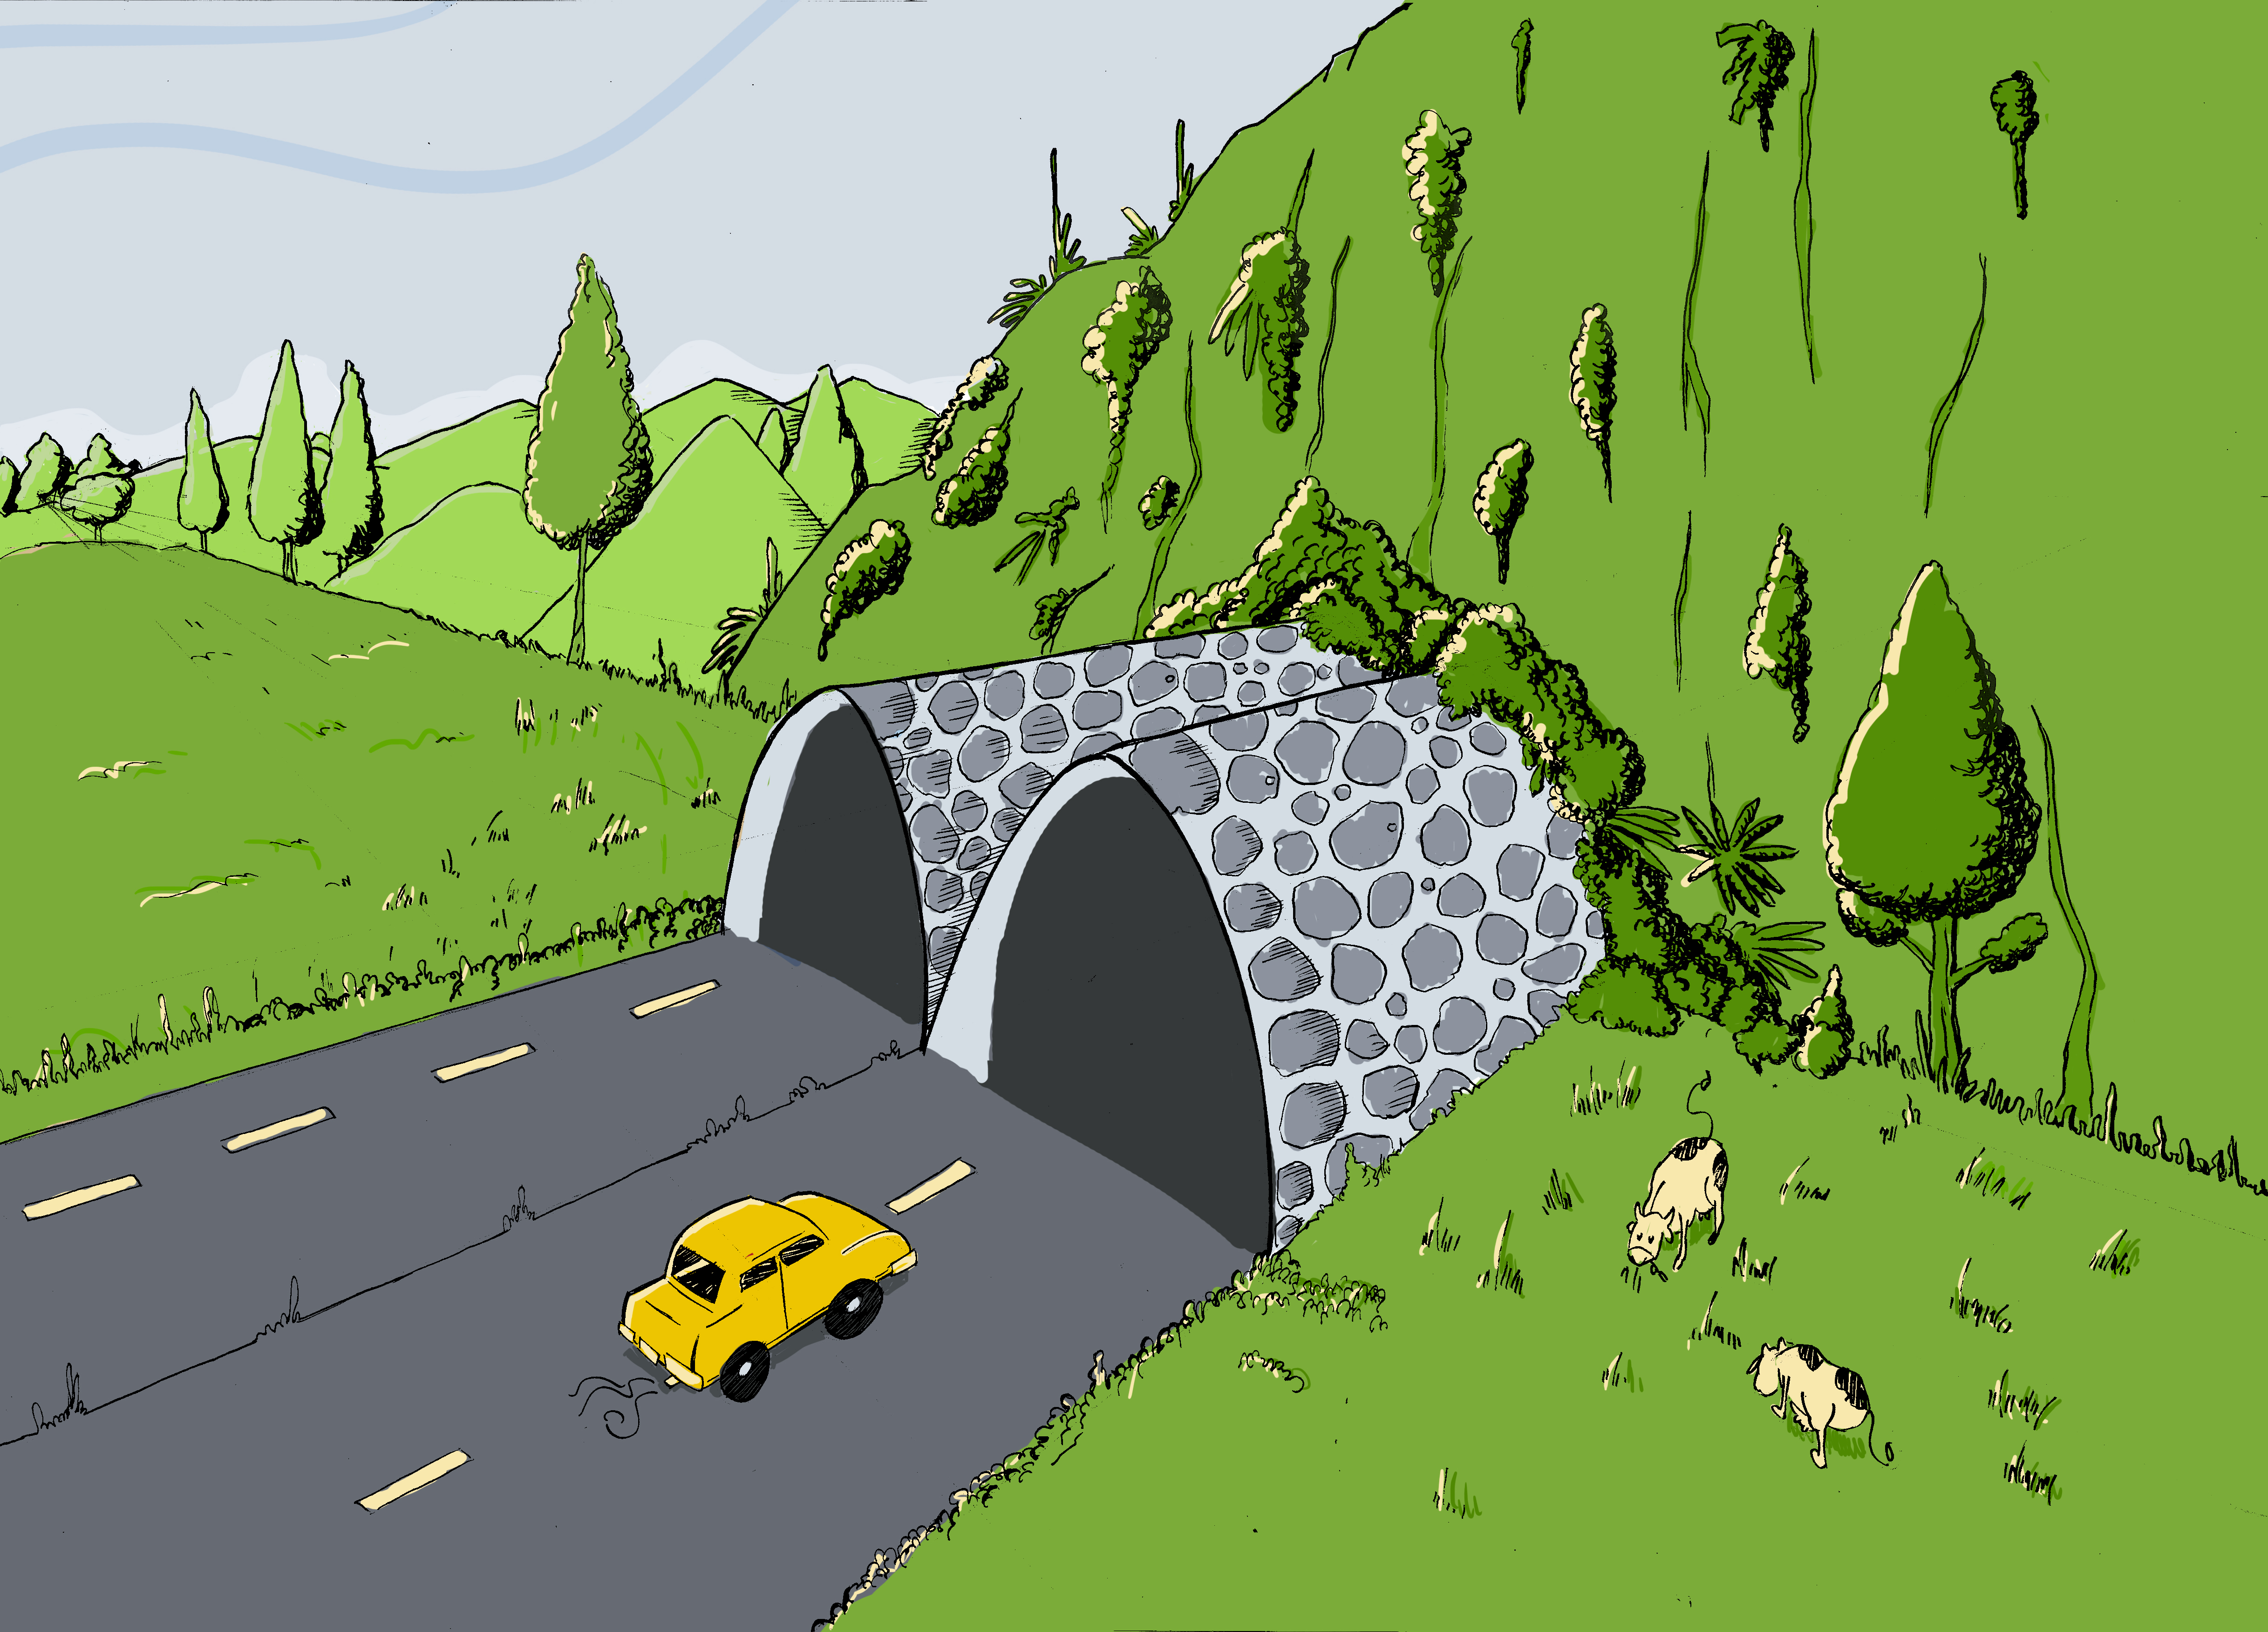
\includegraphics[width=.4\linewidth]{5_1.jpg}
\caption{Exemplo de figura}
\end{figure}

As figuras são em geral centralizadas e podem ou não possuir legenda. Por isso usamos o ambiente de figura dessa forma:

\begin{verbatim}
\begin{figure}[H]
\centering

\includegraphics[width=.4\linewidth]{suafigura.png}
\caption{Legenda}
\label{marcação para referência}
\end{figure}
\end{verbatim}

O ambiente de figura possui uma diferença crucial que é o uso da opção \verb|[H]|. Essa opção é fornecida pelo pacote \verb|float| (incluído no pacote \verb|livroaberto|) e é usada pois a figura não pode estar naturalmente dentro de \href{https://en.wikibooks.org/wiki/LaTeX/Floats,_Figures_and_Captions}{ambiente flutuante}, que é o caso da caixa de atividade, criada por uma \verb|tcolorbox|. Deixamos também a figura, em geral, centralizada.

Pedimos que ao se referir a uma atividade, figura ou tabela utilize \verb|\hyperref[label]{float \ref{label}}|, onde float é substituído por figura, atividade ou tabela, de acordo com a referência. 

\textbf{Atenção}: Os \textit{labels} devem sempre ficar após as \textit{captions} no código, senão o \LaTeX{} não as reconhece propriamente.
\end{task}

\begin{task}{Tabelas}

Tabelas requerem um pouco mais de atenção, pois possuem diversas opções e tipos de construções avançadas. Por isso, recomendamos a leitura do artigo sobre tabelas no \href{https://en.wikibooks.org/wiki/LaTeX/Tables}{Wikibooks}. 

Assim como nas figuras, deve-se usar o parâmetro \verb|H| para que ela funcione normalmente dentro da caixa de atividade. Na nossa padronização de tabela, buscamos um \textit{heading} que possua a mesma cor da parte da seção. Para conseguir isto temos três comandos:

\begin{itemize}
\item \verb|\tcolor{texto}|: Coloca a cor da célula na cor da seção atual e o texto branco em negrito.
\item \verb|\tmcol{#colunas}{alinhamento}{texto}|: Substitui o comando \verb|multicolumn| para ter as características que buscamos na célula.
\end{itemize}

\begin{table}[H]
\centering
\begin{tabular}{|c|c|c|c|}
\hline
\tcolor{Atividade Física} & \tcolor{Manhã} & \tcolor{Tarde} & \tcolor{Total} \\
\hline
\tcolor{Não pratica} & 140 & 130 & 270 \\
\hline
\tmcol{2}{|c|}{Futebol} & 80 & 240 \\
\hline
\end{tabular}
\caption{Versão da tabela usando tabular}
\label{tabela}
\end{table}
\newpage

\begin{verbatim}
\begin{table}[H]
\centering
\begin{tabular}{|c|c|c|c|}
\hline
\tcolor{Atividade Física} & \tcolor{Manhã} & \tcolor{Tarde} & 
\tcolor{Total} \\
\hline
\tcolor{Não pratica} & 140 & 130 & 270 \\
\hline
\tmcol{2}{|c|}{Futebol} & 80 & 240 \\
\hline
\end{tabular}
\caption{Versão da tabela usando tabular}
\label{tabela}
\end{table}
\end{verbatim}

Há também novos tipos de alinhamento de colunas, sendo estes \verb|d|, \verb|e| e \verb|f|.

Estes alinhamentos são implementados pelos seguintes comandos:
\begin{verbatim}
\newcolumntype{d}[1]{>{\vspace{2.5pt}}m{#1}<{\vspace{2.5pt}}}
\newcolumntype{e}[1]{>{\vspace{2.5pt}\centering}m{#1}<{\vspace{2.5pt}}}
\newcolumntype{f}{>$c<$}
\newcolumntype{g}[1]{>$e{#1}<$}
\end{verbatim}
\begin{itemize}
\item O alinhamento \verb|d| é o mesmo que o alinhamento \verb|m|, isto é, especificamos \verb|d{largura}|, onde entre chaves temos a largura de coluna desejada. A diferença dos dois alinhamentos é que é adicionado ao \verb|d| um espaçamento superior e inferior nas células desta coluna, o que é útil em casos que a célula é muito estreita para a entrada.

\item O alinhamento \verb|e| é o mesmo que o alinhamento \verb|d|, a única diferença é que o texto nas células é centralizado.

\item O alinhamento \verb|f| é o mesmo que \verb|c|, mas com todas as células na coluna com o modo matemático.

\item O alinhamento \verb|g| é uma mistura de \verb|e| e \verb|f|
\end{itemize}

Segue um exemplo do uso dos alinhamentos em uma tabela:

\begin{table}[H]
\centering

\begin{tabular}{|d{.15\linewidth}|e{.15\linewidth}|f|g{.15\linewidth}|}
\hline
\tcolor{Espaçamento da coluna \texttt{|d|}} & \tcolor{Espaçamento da coluna \texttt{|e|}} & $\tcolor{Modo matemático \texttt{|f|}}$ & $\tcolor{Modo matemático \texttt{|g|}}$ \tabularnewline
\hline
$\frac{\sqrt{3}}{\sqrt{3}}$ & $\frac{\sqrt{3}}{\sqrt{3}}$ &  \frac{\sqrt{3}}{\sqrt{3}} & \frac{\sqrt{3}}{\sqrt{3}} \tabularnewline
\hline
$\frac{\sqrt{3}}{\sqrt{3}}$ & $\frac{\sqrt{3}}{\sqrt{3}}$ &  \frac{\sqrt{3}}{\sqrt{3}} & \frac{\sqrt{3}}{\sqrt{3}} \tabularnewline
\hline
$\frac{\sqrt{3}}{\sqrt{3}}$ & $\frac{\sqrt{3}}{\sqrt{3}}$ &  \frac{\sqrt{3}}{\sqrt{3}} & \frac{\sqrt{3}}{\sqrt{3}} \tabularnewline
\hline
\end{tabular}
\end{table}

\begin{verbatim}
\begin{table}[H]
\centering
\begin{tabular}{|d{.15\linewidth}|e{.15\linewidth}|f|g{.15\linewidth}|}
\hline
\tcolor{Espaçamento da coluna \texttt{|d|}} & 
\tcolor{Espaçamento da coluna \texttt{|e|}} & 
$\tcolor{Modo matemático \texttt{|f|}}$ &
$\tcolor{Modo matemático \texttt{|g|}}$ \tabularnewline
\hline

$\frac{\sqrt{3}}{\sqrt{3}}$ & 
$\frac{\sqrt{3}}{\sqrt{3}}$ &  
\frac{\sqrt{3}}{\sqrt{3}} & 
\frac{\sqrt{3}}{\sqrt{3}} \tabularnewline
\hline

$\frac{\sqrt{3}}{\sqrt{3}}$ & 
$\frac{\sqrt{3}}{\sqrt{3}}$ &  
\frac{\sqrt{3}}{\sqrt{3}} & 
\frac{\sqrt{3}}{\sqrt{3}} \tabularnewline
\hline

$\frac{\sqrt{3}}{\sqrt{3}}$ & 
$\frac{\sqrt{3}}{\sqrt{3}}$ &  
\frac{\sqrt{3}}{\sqrt{3}} & 
\frac{\sqrt{3}}{\sqrt{3}} \tabularnewline
\hline
\end{tabular}
\end{table}
\end{verbatim}

Neste caso, tanto o alinhamento \verb|d| quanto o \verb|e| ficaram com a largura \verb|.3\linewidth|, isto é, $30\%$ da largura da linha. É possível observar que, no caso da coluna \verb|f|, o alinhamento vertical não é o mesmo das colunas \verb|d| e \verb|f|, não é necessário colocar \$ entre o texto matemático, apenas quando tivemos o texto na primeira linha. Ou seja, usamos os cifrões no sentido contrário, apenas quando queremos escrever textos não-matemáticos. Este modelo de coluna é útil quando se quer escrever colunas em que quase todas as entradas são textos matemáticos. 

\begin{observationtitle}{Observação}
É importante sempre lembrar que ao usar os alinhamentos \verb|e| e \verb|g| como última coluna da tabela, deve-se pular a linha com \verb|\tabularnewline| em vez de \verb|\\|, pois como há o comando \verb|\centering| na sua definição, há problemas em como o \LaTeX{} gera a tabela.
\end{observationtitle}

Por efeito de exemplo, segue abaixo a mesma tabela, mas usando os modelos de coluna original.

\begin{table}[H]
\centering

\begin{tabular}{|m{.15\linewidth}|c|}
\hline
\tcolor{Espaçamento da coluna \texttt{|m|}} & \tcolor{Modo matemático \texttt{|c|}} \\
\hline
$\frac{\sqrt{3}}{\sqrt{3}}$ & $\frac{\sqrt{3}}{\sqrt{3}}$ \\
\hline
$\frac{\sqrt{3}}{\sqrt{3}}$ & $\frac{\sqrt{3}}{\sqrt{3}}$ \\
\hline
\end{tabular}
\end{table}



\begin{verbatim}
\begin{table}[H]
\centering
\begin{tabular}{|m{.15\linewidth}|c|}
\hline

\tcolor{Espaçamento da coluna \texttt{|m|}} & 
\tcolor{Modo matemático \texttt{|c|}} \\
\hline

$\frac{\sqrt{3}}{\sqrt{3}}$ & 
$\frac{\sqrt{3}}{\sqrt{3}}$ \\
\hline

$\frac{\sqrt{3}}{\sqrt{3}}$ & 
$\frac{\sqrt{3}}{\sqrt{3}}$ \\
\hline

$\frac{\sqrt{3}}{\sqrt{3}}$ & 
$\frac{\sqrt{3}}{\sqrt{3}}$ \\
\hline

\end{tabular}
\end{table}
\end{verbatim}

\end{task}



Na caixa anterior temos o "Observação", que pode ser introduzido no texto no ambiente \verb|observationtitle|:
\begin{verbatim}
\begin{observationtitle}{titulo}
Texto da observação
\end{observationtitle}
\end{verbatim}
Ou sua versão sem título:

\begin{verbatim}
\begin{observation}
Para uma versão sem título da caixa de observação pode-se usar o ambiente
\verb|observation| em vez de \verb|observationtitle|
\end{observation}
\end{verbatim}

\begin{observation}
Para uma versão sem título da caixa de observação pode-se usar o ambiente \verb|observation| em vez de \verb|observationtitle|
\end{observation}

Além da caixa de atividade e observação temos mais quatro caixas:

\begin{research}
O "Para pesquisar", feito usando

\begin{verbatim}
\begin{research}
Seu o pesquisar não usa título.
\end{research}
\end{verbatim}
\end{research}

\begin{knowledge}
O "Você Sabia?", que usa o ambiente

\begin{verbatim}

\begin{knowledge}
Esta caixa também não possui título
\end{knowledge}
\end{verbatim}
\end{knowledge}

\begin{reflection}
O Para refletir

\begin{verbatim}

\begin{reflection}
Mais uma caixa que não tem título
\end{reflection}
\end{verbatim}
\end{reflection}

\begin{example}{Exemplo de uma caixa de exemplo}
Por fim, a última caixa é a de exemplo. Caso possua alguma atividade já com a resposta é recomendável usar essa caixa, que pode ser feita com
\begin{verbatim}

\begin{example}{Título}
Esta caixa pede um título, que pode possivelmente ser vazio.
\end{example}
\end{verbatim}
\end{example}

\begin{observation}
As caixas são feitas usando o pacote \verb|tcolorbox|, e é importante ressaltar que este pacote não permite sobrepor caixas, isto é, não se pode colocar uma caixa dentre de outra, e portanto não é possível colcoar uma observação no meio de uma atividade ou semelhantes.
\end{observation}

\arrange{Headers}

Além de boxes, também usamos headers (cabeçalho) para o início de seções. Assim como o explorando é feito com \verb|\explore{nome}|, temos:

\begin{itemize}
\item Organizando: \verb|\arrange{nome}|
\item Praticando: \verb|\practice{nome}|
\item Para saber+: \verb|\know{nome}|
\item Exercícios: \verb|\exercise|
\end{itemize}

Os headers não são ambientes, ou seja, não é necessário um \verb|\begin| e \verb|\end|, pois funcionam como seções novas. 

Uma característica interessante é a mudança de cores do texto em relação ao header, que faz justamente a mudança das cores de células das tabelas que vimos anteriormente

\begin{table}[H]
\centering
\begin{tabular}{|c|c|c|c|}
\hline
\tcolor{Atividade Física} & \tcolor{Manhã} & \tcolor{Tarde} & \tcolor{Total} \\
\hline
\tcolor{Não pratica} & 140 & 130 & 270 \\
\hline
\tmcol{2}{|c|}{Futebol} & 80 & 240 \\
\hline
\end{tabular}
\caption{Exemplo da mudança de cor}
\label{frequenciaatividade}
\end{table}


\practice{Outros tipos de padrões}

\begin{task}{Padrões no texto}
Colocamos sempre letras representando variáveis e conjuntos no modo de matemática. Números quando se referem a equações e unidades de medida, porcentagem e valores monetário também ficam em texto matemático. Porcentagens são escritas por \verb|$70\%$|, unidades de medida são do modo \verb|$70$mm|, e valores monetários \verb|R\$ $70$|, por exemplo.

O \LaTeX{} usa o sistema americano para casa decimais, e sempre coloca um espaço após a vírgula. Como aqui números decimais ficam após uma vírgula, é necessário usar \verb|{,}| para que não haja esse espaço (o espaço deve existir em outros casos, como pares ordenados e afins). Usamos também o padrão de pontos separando milhares, isto é, escrevemos 1.000.00 para representar um milhão.
\end{task}

\begin{task}{Bibliografia}
Para a formatação da bibliografia utilizamos o modelo BibTeX. Para inserir a bibliografia do seu capítulo, ou para editá-la, ela deve estar na pasta \verb|Bibliografia/| no formato \verb|nomedocapitulo_bibliografia.bib|. Ao final do capítulo, deve haver a linha \verb|\bibliography{../Bibliografia/nomedocapitulo_bibliografia.bib}|. A compilação da bibliografia deve ser feita utilizando o comando, dentro da pasta \verb|chapters/|, e após ter compilado o capítulo ao menos uma vez:

\begin{verbatim}

bibtex nomedocapitulo
\end{verbatim}
A bibliografia aparecerá na próxima compilação do capítulo.
\end{task}

\begin{knowledge}
É possível encontrar modelos de Bibliografia em BibTeX no site \href{https://verbosus.com/bibtex-style-examples.html}{Verbosus}.
\end{knowledge}

\exercise

\begin{enumerate}
\item A seção de exercícios não possui título, e é feita usando o ambiente \verb|enumerate|.
\begin{enumerate}
\item É possível colocar enumerações
\begin{enumerate}
\item Em cima de numerações
\begin{enumerate}
\item Mas no momento apenas três níveis possuem \textit{labels}.
\end{enumerate}
\end{enumerate}
\end{enumerate}

\item E então pode continuar até onde for desejado.
\end{enumerate}

O ambiente a seguir é o de projeto aplicado
\begin{verbatim}
\begin{project}
o projeto aplicado não possui título
\end{project}
\end{verbatim}

\begin{project}
Este é ambiente para criação de um projeto aplicado. Ele cria uma nova página exclusiva para ele

\end{project}

% \begin{paginatexto}{Página de texto no meio do capítulo}
% \label{paginatexto}
% Para fazer uma transição entre seções de um capítulo é possível utilizar o ambiente \verb|paginatexto|, que possui o mesmo funcionamento do ambiente de apresentação. Suas únicas diferenças são a cor do realçamento e a paginação. Este ambiente não altera a paginação no meio do texto, isto é, a página após este ambiente continuará com a numeração seguinte à que precede estas páginas. Esta escolha foi feita para que o material do professor tenha a paginação igual ao do material do aluno. O ambiente é definido como

% \begin{verbatim}
% \begin{paginatexto}{Título}

% \end{paginatexto}
% \end{verbatim}
% \end{paginatexto}

\know{Sintaxe do Livro Aberto}

Aqui vamos falar um pouco da estrutura dos capítulos do Livro Aberto do Ensino Médio.

Todo capítulo começa em sua capa com 

\begin{itemize}
\item uma breve descrição do assunto do capítulo (\textbf{O quê?})
\item uma justificativa para o estudo no capítulo (\textbf{Por quê?}).
\end{itemize} 

\subsection{Para o professor (do capítulo)}
Após a página com os créditos, o capítulo começa com um "Para o professor" que versará sobre o capítulo inteiro, isto é, uma apresentação para os docentes sobre o que trata o capítulo e como deve ser trabalhado. O "Para o professor" do capítulo deve conter:

\begin{itemize}
\item Habilidades da BNCC ou extras que estão sendo contempladas.
\item Listar os conceitos e fatos matemáticos contidos no capítulo.
\item Destacar e justividar os conceitos e fatos que tradicionalmente são ensinados e que decidiu-se não ensinar no capítulo.
\item Destacar o percurso pedagógico a partir da estrutura de seções do capítulo.
\item Apresentar os pré requisitos para o capítulo.
\item O que há de inovador no capítulo em relação aos materiais didáticos correntes.
\item Citar a bibliografia utilizada e que serviu de base para as decisões na construção do material ao longo deste texto e as referências no final do mesmo.
\end{itemize}

\subsection{Seção}

Cada seção possui a seguinte estrutura:

\subsection{Para o professor (da seção)}
Este "Para o professor"{} deve conter:
\begin{itemize}
\item Lista de Objetivos Específicos de Aprendizagem da seção.
\item Conhecimento Pedagógico do assunto: Matemática subjacente, que eventualmente não seja explicitada aos estudantes, mas que seja utilizada como base da seção (opcional).
\item Apresentação do percurso pedagógico da seção, explicando a linguagem, o que espera-se ensinar nesta seção e o que espera-se que não seja ainda discutido.
\end{itemize}

\def\currentcolor{session1}
\subsection{Explorando: Título da seção}

Aqui são colocadas as atividades de exploração do assunto, ou seja, atividades que consigam refletir o que será tratado na seção. É opcional possuir um texto introdutório (mas desejado).

As atividade também devem possuir um "Para o professor", este que deve conter:
\begin{itemize}
\item Objetivos Específicos de Aprendizagem.
\item Sugestões e discussões, como: organização da turma; tempo estimado; conceitos abordados; linguagem; dificuldades previstas; sugestões gerais; enriquecimento da discussão; conexões; material necessário (os itens são opcionais e variam de acordo com a necessidade da atividade).
\item Solução completa.
\end{itemize}

\def\currentcolor{session4}
\subsection{Organizando: Título da seção}

No Organizando colocamos a sistematização do conteúdo da seção, formalizando os conceitos que foram investigado pelos alunos anteriormente. É recomendado colocar exemplos para a melhor compreensão do aluno.

\def\currentcolor{session2}
\subsection{Praticando: Título da Seção}

Aqui são colocadas mais atividades que complementem a seção. O praticando é opcional.

\def\currentcolor{primario}
\subsection{Exercícios}

Os exercícios no final da seção são também opcionais. Deve também conter um para o professor do exercício, que deve onter os Objetivos Específicos de Aprendizagem e a resposta ou solução (curta).


Ao fim de todas as seções do capítulo, é necessário que haja exercícios que reflitam o conteúdo do capítulo. Além dos exercícios, é opcional haver o \textcolor{session3}{\textbf{Para Saber+}} e o \textcolor{cor2}{\textbf{Projeto Aplicado}}.

\def\currentcolor{session3}
\subsection{Boxes}

Os boxes podem ser posicionados nas seções Explorando, Organizando as Ideias ou Praticando, mas é importante que respeitem as seguintes orientações:

\begin{observationtitle}{Observação}
Esta caixa é essencial. Serve para destacar comentários fundamentais para o desenvolvimento do estudante ou para o aprendizado do conteúdo. Sua leitura é obrigatória.
\end{observationtitle}
\clearpage
\begin{reflection}
A caixa "Para refletir"{} é importante, mas não essencial. Convida o estudante a uma reflexão adicional ou de aprofundamento. Pergunta, afirmação ou curiosidade. A leitura é recomendada.
\end{reflection}

\begin{knowledge}
Esta caixa é para aprofundamento. Não traz grande prejuízo para o cumprimento da habilidade proposta se o estudante pular estas caixas. É uma espécie de "Para saber mais"{ curto que pode ser usado nas demais seções}.

Curiosidades sobre conceitos, propriedades ou termos utilizados, usos dos conceitos em outros contextos, conexão com outras áres do conhecimento ou da própria matemática, etc.
\end{knowledge}


\ifnum\aluno=1
\clearpage
\else
\notasfinais
\fi